As per the literature I read during the initial part of my internship, I designed a generalised circuit (Figure \ref*{fig:f-gain-circuit}) that takes just the basic required paramteres of any LLC Converter, and calculates the rest accordingly, and give us the theoritical plot of the frequency-gain curve of the converter, which mostly coincides with the actual plot of the gain v/s frequency as well. (Verified that experimentally by measuring the frequencies at multiple points and calculating the gain of the LLC tank at that instant and plotting it against the frequency at that instant)
\begin{figure}[H]
    \centering
    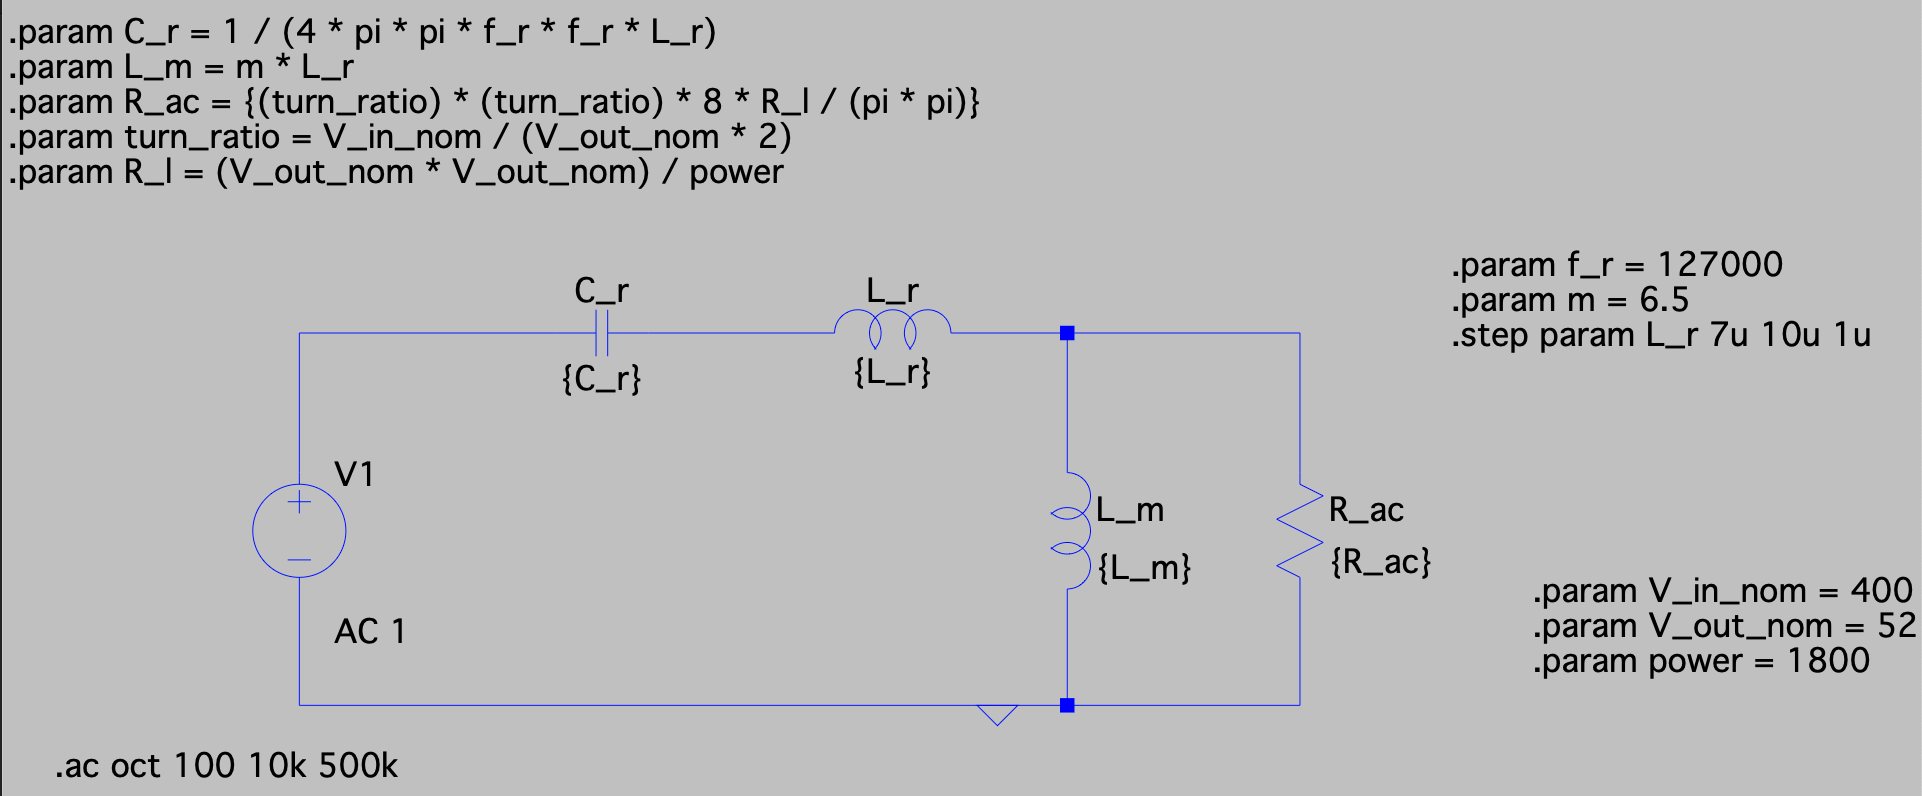
\includegraphics[width=\textwidth]{f-gain-circuit.png}
    \caption{Schematic of the frequency-gain curve plotter}
    \label{fig:f-gain-circuit}
\end{figure}

\begin{itemize}
    \item The bottom-right parameters are from the required specifications, i.e., the nominal input volage, nominal output voltage, and the rated maximum power of the converter.
    \item The centre-right parameters are of the resonant frequency that we want for our design (usually 100-150 kHz for a SMPS), the value of $m$ (The ratio of magnetizing inductor to the series inductor = $L_m / L_r$)
    \item The .step parameter is used to generate multiple graphs at the same time with different specs (for example, the given graph (Figure \ref*{fig:f-gain-out}), shows multiple graphs for different combinations of LLC simultaneously). This helps in fine-tuning the values according to our gain requirements.
    \item The top-left parameters are equations and other variables that are dependent on the values that we give as input.
    \item The bottom-left parameter is the range of frequencies between which we want to plot the graph. (As per the current circuit, between 10kHz to 500kHz with step size of 100Hz)
\end{itemize}
\begin{figure}[H]
    \centering
    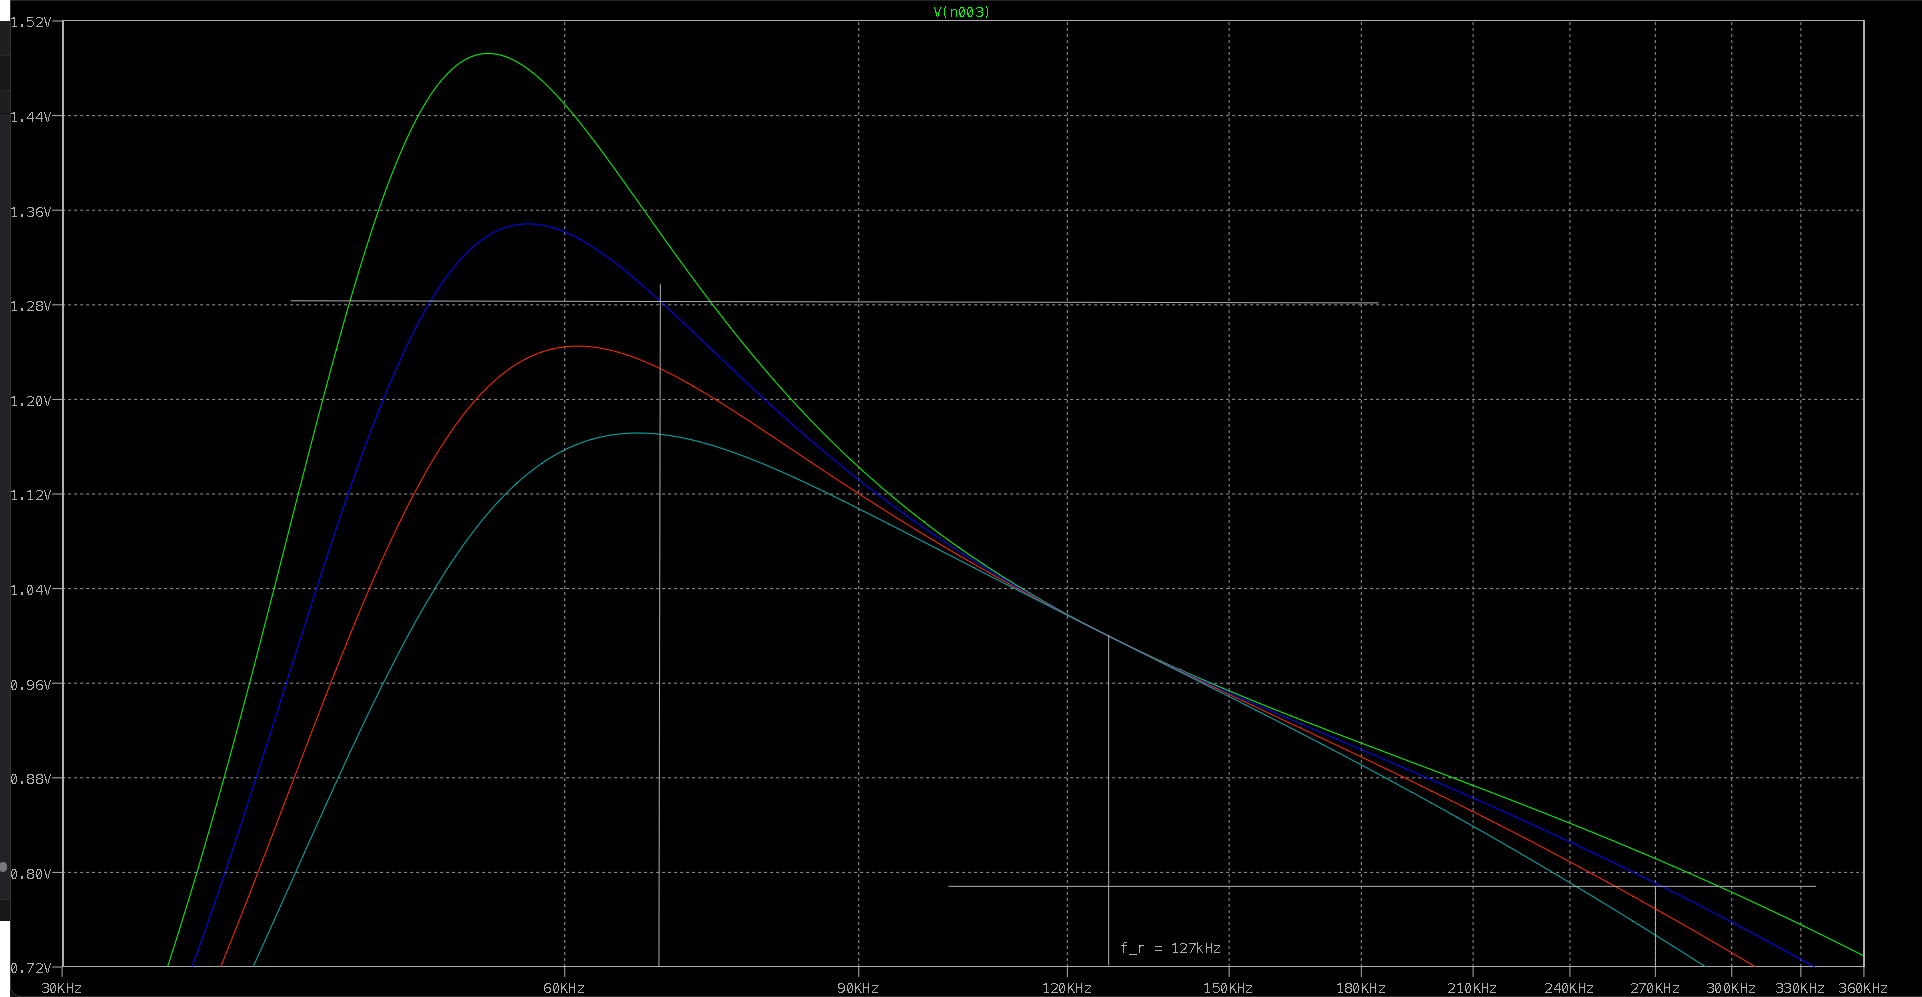
\includegraphics[width=\textwidth]{f-gain-out.png}
    \caption{Output of the frequency-gain curve plotter}
    \label{fig:f-gain-out}
\end{figure}